GATE Teamware  is a software suite and a methodology for the implementation and
support of \emph{annotation factories}: it is intended to provide a framework
for commercial annotation services, supplied either as in-house units or as
outsourced specialist activities. This framework is a novel development in
several aspects:
\begin{itemize}
  \item it structures intervention by different actors (human and machine)
  into clearly-defined roles and provides the means to manage them in a
  unified fashion,
  \item it complements GATE's developer-oriented facilities with User
  Interfaces (UIs) oriented on other necessary staff roles,
  \item it is methodological instead of purely technological.
\end{itemize}

\section{Roles}
There are a number of staff roles required for an effective annotation factory
including:
\begin{itemize}
  \item \textbf{annotators}, who are largely unskilled, may be
  geographically distributed, and whose work is quality controlled by curators
  via metrics-related mechanisms,
  \item \textbf{curators}, who may be skilled annotators, capable of making
  decisions and valuing annotator's work,
  \item \textbf{language engineers}, these staff work on resources producing
  automatic annotations. These resources are combined to produce a service.
  \item \textbf{managers}, who are supposed to create and manage annotation
  projects
  \item \textbf{administrators}, who administrate the workflow system and its
  users.
  \item \textbf{superadministrator}, single super user who can modify the
  critical parts of the application along with other administrator
  duties 
\end{itemize}
GATE Teamware, together with GATE Developer, provides tools for all these roles,
and the workflow by which they may be combined with automatic Information Extraction
(IE) systems to provide cost-effective annotation services.

\section{Prerequisites}
GATE Teamware is a Java web application deployable under Apache Tomcat server
(5.5.x and 6.x) and fully compatible with both JDK 1.5 and 1.6. 
Apart from a web browser (the currently supported versions are Internet
Explorer (versions: 6, 7 and 8), Firefox 1.5, 2.x, 3.x) and Opera (versions: 8,
9 and 10)) you need to have Java Web Start (JWS) version 1.6.0 installed on
client machines. JWS can be downloaded as the part of Java Runtime Environment
(JRE) version 6 from the following address:
\url{http://java.sun.com/javase/downloads/index.jsp}

\section{Login}
GATE Teamware authentication and authorisation is accomplished twofolds:
\begin{itemize}
  \item through Database
  \item through Active Directory (AD), so that all users who have AD account can
  log in to the GATE Teamware with the same credentials. The scenario supported at
the moment is:
\end{itemize}

By default the authentication and authorisation are performed against database.
New user gets registered:
\begin{itemize}
  \item either by following \emph{Signup} link at the login page (see
  Figure~\ref{fig:login-page})
  \item  or by administrator, who also assigns role(s) to the new user. 
\end{itemize}

With AD situation is a bit more complicated. The following scenario applies:

\begin{itemize}
\item when the AD user signs in for the first time, s/he will be added to
Teamware database (DB) with the appropriate role; currently, these roles are \emph{manager},
\emph{curator} and \emph{annotator}; this can be changed in administration section
later.
\item the user profile in the GATE Teamware DB is automatically populated by
matching data from AD account. All other data have the default values, which can be
changed later.
\end{itemize}

When you type teamware url like
\url{http://[host.name]:[host.port]/[instance.name]/executive} in your browser, you will be prompt with the login page, see Figure~\ref{fig:login-page}.

\begin{figure}[htb]
\centering
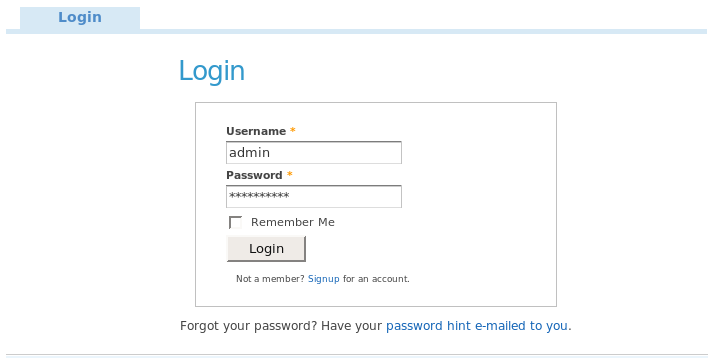
\includegraphics[scale=0.5]{login}
\caption{Login Form}\label{fig:login-page}
\label{fig:login}
\end{figure}

Login with your username and password.

\section{Home Page}
After you have logged in successfully, you will be redirected to your
\emph{home page}. The menu items differ based on the type of the user role. If
logged in as a \emph{manager}, you should see the menu and shortcut links as
shown in Figure~\ref{fig:manager-home-page}. For users with annotator roles,
the number of available options will be reduced (e.g., the menus
\emph{Resources} and \emph{Projects} will not be visible).
\begin{figure}[htb!]
\centering
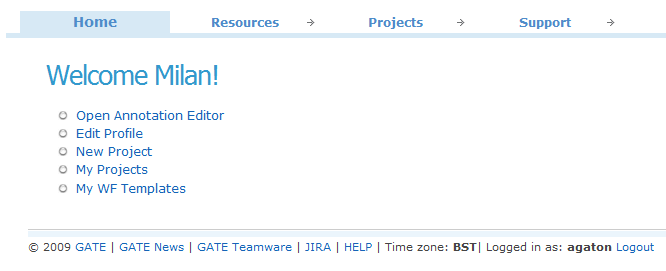
\includegraphics[scale=0.5]{main}
\caption{Home Page - Example}
\label{fig:main}
\end{figure}

\section{Edit Profile}
You can access/change your profile by clicking on \emph{Edit Profile} link from
the home page (see Figure~\ref{fig:main}). The
\emph{Edit Profile} form as shown in Figure~\ref{fig:editprofile}.
\begin{figure}[ht!]
\centering
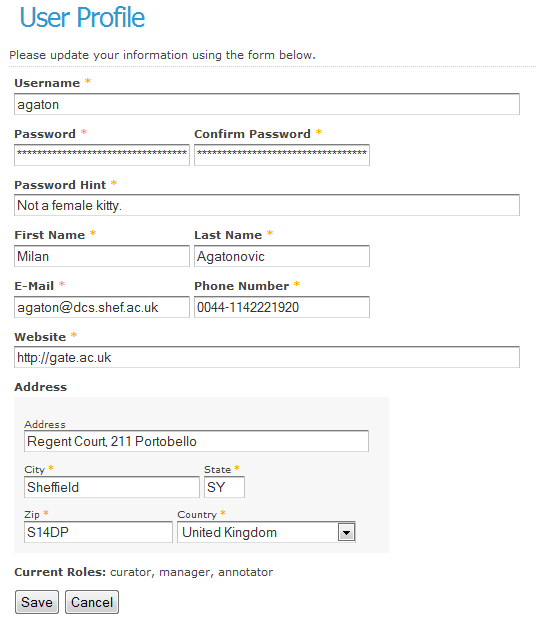
\includegraphics[scale=0.5]{editprofile}
\caption{Edit Profile}
\label{fig:editprofile}
\end{figure}

Note that, in case of AD authentication, only those fields which exist in your
AD profile will be copied to your GATE Teamware profile (see Table~\ref{tab:fields}). Other field values
will be provisional and you should change them after the first login.

\begin{table}[ht!]
\vspace{0mm}
\begin{center}
\caption{The overview of matched fields in AD and Teamware DB}
\vspace{2mm}
\small
\label{tab:fields}
\begin{tabular}{ | l | l |}
\hline
\textbf{Active Directory attribute name} &
 \textbf{Teamware DB Field Name} \\ \hline  \hline

\emph{givenName} & \emph{first\_name}\\
\hline
 \emph{sn} & \emph{last\_name}\\
\hline
 \emph{sAMAccountName} & \emph{username}\\
\hline
\emph{msSFU30Password} & \emph{password}\\
\hline
\emph{mail} &    \emph{email}\\
\hline
\emph{telephoneNumber} & \emph{phone\_number}\\
\hline
  \end{tabular}
\normalsize{}
\end{center}
\vspace{-5mm}
\end{table}

\section{Logout}
When you finish your session, click on \emph{logout} link in the bottom-right
corner.